\section{Introduction}\label{sec:Introduction} \label{sec:Intro}
%%%%%%%%%%%%%%%%%%%%%%%%%%%%%%%%%%%%%%%%%%%%%%%%%%%%%%%%%%%%%%
The electron drift time (and by extension the drift velocity) is a fundamental parameter to the working principal of a LArTPC. By knowing the speed of the electron drift we are able to project the position of the charge back into the TPC volume enabling 3D reconstruction. The drift velocity is determined by the electric field in the drift volume, so having a good handle on the electric field is essential. In this note, we present two methods to calculate the electric using the measured detector properties such as temperature, pressure, voltage and current of the LArIAT TPC during its operation in Run-I, II, and III.

We first define some of the basic working parameters of the LArIAT experiment in Section \ref{sec:Def} and then move on showing two methods of calculating the electric field expected in the drift volume. In Section \ref{sec:elDiagram} we use the simple single line diagram of the electric circuit along with the values recorded in ACNET to calculate the voltage on the cathode. Using this voltage we then calculate the electric field, drift velocity, and drift time. In Section \ref{sec:CAMethod} we use an alternative method by identifying cathode to anode piercing tracks (tracks which cross the cathode and wire planes as they traverse the TPC) to calculate the drift time. From this drift time, the drift velocity is calculated, and finally the electric field. 

These two methods give consistent results to one another giving us confidence that we understand the electric field present in the drift volume.

%%%%%%%%%%%%%%%%%%%%%%%%%%%%%%%%%%%%%%%%%%%%%%%%%%%%%%%%%%%%%%%%%%%%%%%%%%%%%%%%%
\subsection{Definitions: electric field, drift velocity and drift time }\label{sec:Def}
%%%%%%%%%%%%%%%%%%%%%%%%%%%%%%%%%%%%%%%%%%%%%%%%%%%%%%%%%%%%%%%%%%%%%%%%%%%%%%%%%
As shown in Figure \ref{fig:driftregions}, the LArIAT TPC has three drift volumes, each of which has its own electric field defined in that region. The main drift volume is defined as the region between the cathode and the uninstrumented shield plane (C-S). This is the region for which the majority of this note will be focused on when calculating the electric field, drift velocity, and drift times.

The other two drift regions are those between the shield plane and the induction plane (S-I), and the region between the induction plane and the collection plane (I-C). The electric field in these regions is chosen to satisfy the charge transparency condition to allow for 100$\%$ transmission of the drifting charge from the drift region to the collection plane.

\begin{figure}[htb]
\centering
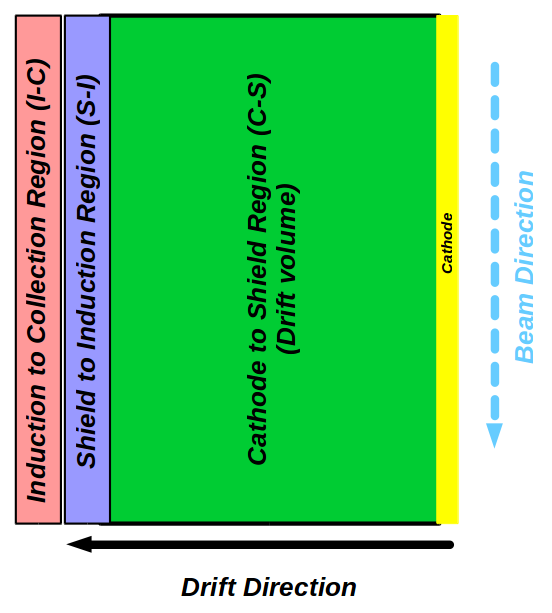
\includegraphics[scale=0.35]{./images/DriftRegions.png}\\
\caption{Schematic of the three drift regions inside the LArIAT TPC. The main drift volume between the cathode and the shield plane (C-S), the region between the shield plane and the induction plane (S-I), and the region between the induction plane and the collection plane (I-C).}
\label{fig:driftregions}
\end{figure}

Table \ref{tab:voltages} provides the voltages applied to the shield, induction, and collection plane for Run-I, and Run-II. These voltages were changed in Run-III, but the transparency condition is was still maintained. For data taken in Run-I and Run-II the spacing between the S-I and I-C regions was a constant 4~mm.

\begin{table}[htpb]
\centering
\caption{Anode planes voltages}
\label{tab:voltages}
\begin{tabular}{lll}
\hline
\multicolumn{1}{|l|}{VShield} & \multicolumn{1}{l|}{VInduction} & \multicolumn{1}{l|}{VCollection} \\ \hline
\multicolumn{1}{|l|}{-298.75} & \multicolumn{1}{l|}{-18.5}      & \multicolumn{1}{l|}{338.5}       \\ \hline
                              &                                 &                                 
\end{tabular}
\end{table}

Once we have the electric field we can calculate the drift velocity ($v_{drift}$) using the relationship
\begin{equation} v_{drift} = \mu(E_{field},T) E_{field}, \label{eq:vd}
\end{equation}
where where $\mu$ is the electron mobility and depends on the electric field and the temperature (T). The emperical formula for this dependency is described in ~\cite{WWW} and shown in Figure \ref{fig:EV} for several argon temperatures.

\begin{figure}[htb]
\centering
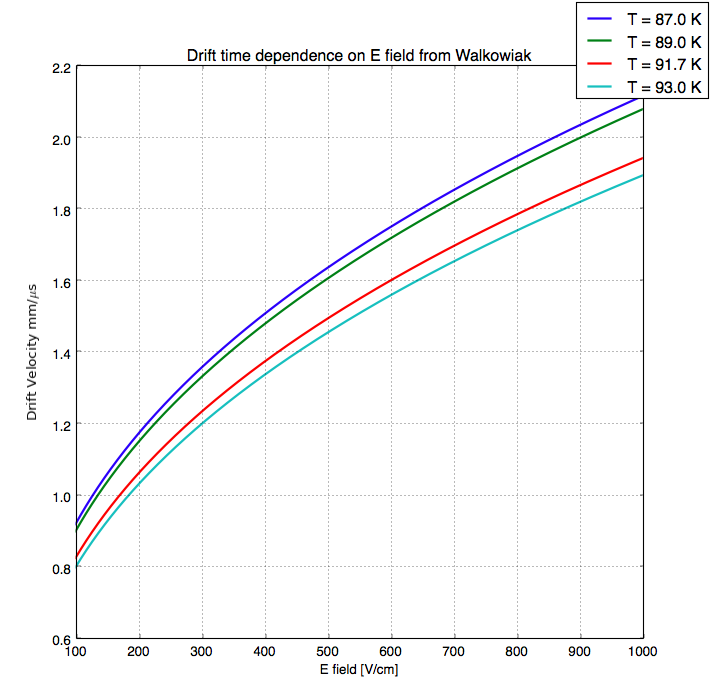
\includegraphics[scale=0.45]{./images/Walkowiak.png}\\
\caption{Drift velocity dependence on electric field for several temperatures. The slope of the line at any one point represents the electron mobility for that given temperature and electric field.}
\label{fig:EV}
\end{figure}

To calculate the electric field in the S-I and I-C regions we can utilize the equation
\begin{equation} E_{field}=\frac{\Delta V_{ab}}{\Delta x}, \label{eq:Efield}
\end{equation}
where $\Delta V_{ab}$ is the voltage difference between two consecutive regions and $\Delta x$ is their spacing.

Table \ref{tab:Efields} reports the values of the electric field, drift velocity and drift times for the smaller drift volumes; the next few paragraphs describe how these quantities are calculated.

  

The electric field is calculated using equation \ref{eq:Efield}:







 
\begin{table}[]
\centering
\caption{Electric field and drift velocities in LArIAT smaller drift volumes}
\label{tab:Efields}
\begin{tabular}{|l|l|l|}
\hline
& Shield-Induction & Induction-Collection \\ \hline
E$_{filed}$ &                 700.625 V/cm        &                892.5  V/cm             \\ \hline
v$_{drift}$ &                   1.73  mm/$\mu$s   &                  1.90 mm/$\mu$s        \\ \hline
t$_{drift}$ &                   2.31  $\mu$s      &                   2.11 $\mu$s          \\ \hline

\end{tabular}
\end{table}

From the electric field, we calculate the drift velocity and substquently the drit time in the volumes bewteen shield and induction planes and induction and collection planes.
The relationship between drift time and drift velocity is straightforward 
\begin{equation}
v_{drift} = \Delta x/t_{drift}, \label{eq:drifttime}
\end{equation}
but the one between  electric field and drift velocity is more complicated. The relationship between the electric field and drift velocity in LAr can be described as 






In order to determine the temperature inside the TPC, we use the measurement of the pressure at the top of the cryostat. This pressure is maintained constant at ~20 psi at the liquid argon surface (PT219A in figure \ref{fig:cryo}). Figure \ref{fig:pressure} shows the distribution of the pressure reading for 13 days.
The average pressure is 20.0 $\pm$ 0.4 psi,  which corresponds to argon temperature of  90.328K  according to NIST RefProp [\textcolor{red}{reference}]. In order to calculate the pressure (and subsequently the temperature) in the middle of the TPC, we consider about 40 cm of Argon from the lulage surface. This argon raises the pressure of about 0.79 psi in the middle of the TPC. A pressure of ~20.79 psi corresponds to a temperature to ~90.7 K according to NIST. We'll assume a temperature of 90.7 K for the rest of the note.

It should be noted that LArIAT is equipped with three temperature probres inside the LAr: one at the bottom (TE213A in figure \ref{fig:cryo}), one in the middle (TE314A in figure \ref{fig:cryo}) and one on the top of the cryostat (TE212A in figure \ref{fig:cryo}). These probes have a similar temperature reading (see \ref{tab:temp}), but since they were not calibrated we prefer to rely on the pressure measurement.

 %\textcolor{red}{On average}, the three probes read as shown in table \ref{tab:temp}. 
\begin{table}[]
\centering
\caption{Average temperatures measured at the top, middle and bottom in the LArIAT cryostat.}
\label{tab:temp}
\begin{tabular}{|c|c|c|}
\hline
Top Probe Temp (TE212A) & Middle Probe Temp (TE214A)   & Bottom Probe Temp (TE213A)  \\ \hline
91.7 $\pm$ 0.7 K &  91.8 $\pm$ 0.7 K                   & 93.3 $\pm$ 2.7 K       \\ \hline
\end{tabular}
\end{table}


\begin{figure}[ht!]
\centering
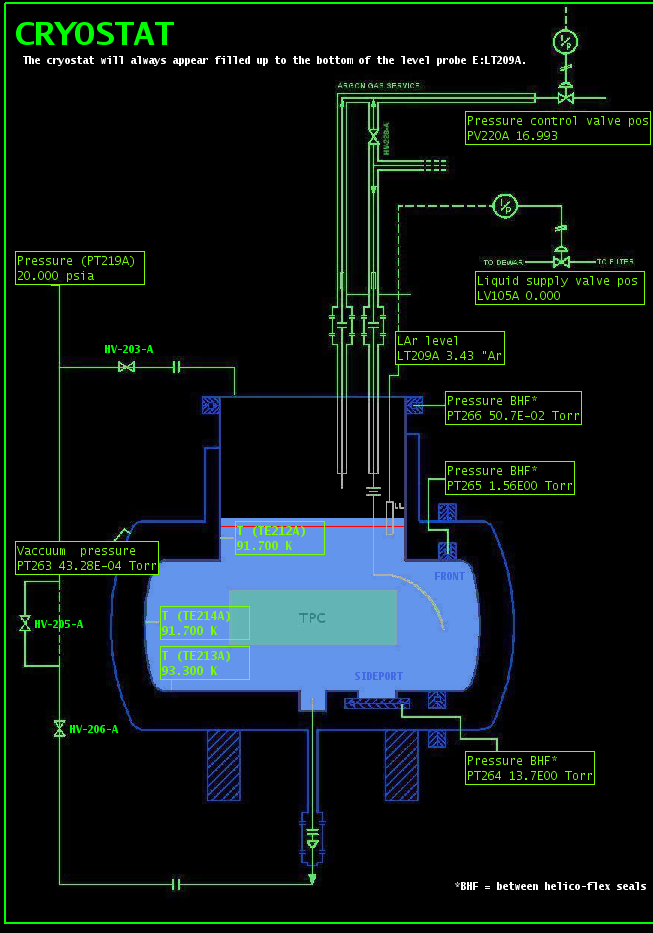
\includegraphics[scale=0.45]{./images/cryopic.png}\\
\caption{Scheme of LArIAT cryostat and cryo probes.}
\label{fig:cryo}
\end{figure}


\begin{figure}[ht!]
\centering
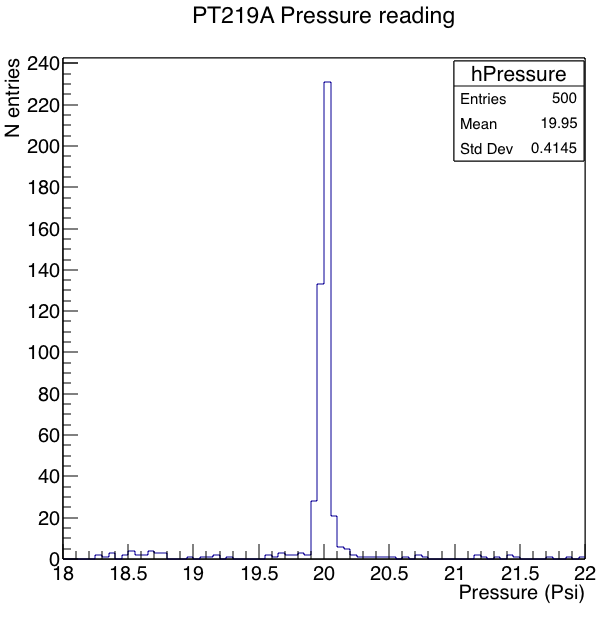
\includegraphics[scale=0.45]{./images/Pressure.png}\\
\caption{PT219A pressure distributions for 13 days (2017/6/23 - 2017/7/5).}
\label{fig:pressure}
\end{figure}





